\documentclass[12pt]{article}
%Also I made it 12pt

\usepackage[fontset=macnew]{ctex}
\usepackage{physics}
\usepackage{tikz}
\usetikzlibrary{3d,calc,patterns,chains,arrows.meta, positioning}
% \usepackage{tkz-euclide}
\usepackage{amsmath}
\usepackage{upgreek}
\usepackage{amsthm}
\usepackage{amsfonts}
%to add an affiliation line to the the title formatting
\usepackage{authblk}

%Fonts
% \usepackage[no-math]{fontspec} %This allows you to enter (via an IPA kayboard) IPA fonts and other symbols directly into LaTeX. Requires a particular setyp, see below.
\usepackage{libertine} %A font that actually contains many IPA symbols. This is the font you see in the preview to the right.

%to use these fonts, be sure that your typesetting engine is set to "XeLaTeX." In Overleaf, go to the Menu link on the top left (by the Overleaf icon), and under Settings be sure that the Compiler is set to "XeLaTeX." If you accessed this document via the Overleaf Pomona Linguistics template, all of this was already done for you.

%The Pomona Linguistics Paper Template in Overleaf is already set up for this, but you may run into this problem if you start building your own documents.


%%%%%%%%%%%%%%%%%%%%%%%%%%%%%%%%%%%%%%%%%%%%%%%%%%%
%packages for this style of handout-formatting of (sub)section headers 
\usepackage[explicit]{titlesec}
\usepackage{xcolor}

\definecolor{light-gray}{gray}{0.7}
\definecolor{lighter-gray}{gray}{0.85}

\titleformat{\section}
{\normalfont\Large\bfseries}{}{0em}{\colorbox{black}{\parbox{\dimexpr\textwidth-2\fboxsep\relax}{\textcolor{white}{\thesection\quad#1}}}}

\titleformat{\subsection}
{\normalfont\large\bfseries\scshape}{}{0em}{\colorbox{light-gray}{\parbox{\dimexpr\textwidth-2\fboxsep\relax}{\textcolor{black}{\thesubsection\quad#1}}}}

\titleformat{\subsubsection}
{\normalfont\bfseries}{}{0em}{\colorbox{lighter-gray}{\parbox{\dimexpr\textwidth-2\fboxsep\relax}{\textcolor{black}{\thesubsubsection\quad#1}}}}
%%%%%%%%%%%%%%%%%%%%%%%%%%%%%%%%%%%%%%%%%%%%%%%%%%%

%%% This file is the preamble for the Pomona Linguistics LaTeX Paper Template, which is also used for the Quick Reference Guide. If you are brand new to writing with LaTeX, we suggest NOT messing with it, and just writing your paper using the Paper Template. If you are getting more comfortable in LaTeX and want to add packages and commands, this is where you do it (when using this template).

%For stacking text, used here in autosegmental diagrams
\usepackage{stackengine}

%To combine rows in tables
\usepackage{multirow}

%geometry helps manage margins, among other things.
\usepackage[margin=1in]{geometry}

%Gives some extra formatting options, e.g. underlining/strikeout
\usepackage{ulem}

%For putting links into papers, also helps make cross-references in the paper smart references
\usepackage[colorlinks = true,
            linkcolor = blue,
            urlcolor  = blue,
            citecolor = blue,
            anchorcolor = blue]{hyperref} %smarter cross-references, these options turn links blue

%Use package/command below to create a double-spaced document, if you want one. Uncomment BOTH the package and the command (\doublespacing) to create a doublespaced document, or leave them as is to have a single-spaced document.
%\usepackage{setspace}
%\doublespacing 

%paragraph formatting
\usepackage[parfill]{parskip}
\setlength{\parskip}{5pt} %plus 1 minus 1}
\setlength{\parindent}{30pt}
\usepackage{titlesec}

%use for special OT tableaux symbols like bomb and sad face. must be loaded early on because it doesn't play well with some other packages
\usepackage{fourier-orns}

%Basic math symbols 
\usepackage{pifont}
\usepackage{amssymb}

%%%Gives shortcuts for glossing. The use of this package is NOT explained in the Quick Reference Guide, but the documentation is on CTAN for those that are interested. MJKD finds it handy for glossing. (https://ctan.org/pkg/leipzig?lang=en)
\usepackage{leipzig}

%Tables
\usepackage{caption} %For table captions
\usepackage{booktabs} %helps format tables

%For citations and bibliography - as of 9.1.2019 we don't explain citations in this Quick Reference Guide, but Pedro Martin's tutorial does (see links in the Guide).
\usepackage{natbib}

%For OT-style tableaux
\usepackage{ot-tableau}

%highlights text with \hl{text}
\usepackage{color, soul}

%Drawing Syntax Trees
\usepackage[linguistics]{forest}

%This specifies some formatting for the forest trees to make them nicer to look at
\forestset{
  nice nodes/.style={
    for tree={
      inner sep=0pt,
      fit=band,
    },
  },
  default preamble=nice nodes,
}

%% For numbered and glossed examples %%
\usepackage{gb4e}



%Changes the \maketitle command to be smaller and take up less space on a page. 
\makeatletter         
\def\@maketitle{   % custom maketitle 
\noindent {\Large \bfseries \color{black} \@title}  \\ \hrule \noindent \@author \\ \@date  
}

%The code below will draw a circle around a piece of text. This is very useful for drawing attention to a word in a data example. use the command \circled{text} where the argument (`text' here) is what you want to be circled. This is illustrated in the Quick Reference Guide and the Paper Template.

\usepackage{tikz}

\newcommand{\circled}[1]{\begin{tikzpicture}[baseline=(word.base)]
\node[draw, rounded corners, text height=8pt, text depth=2pt, inner sep=2pt, outer sep=0pt, use as bounding box] (word) {#1};
\end{tikzpicture}
}


%%%%%%%%%%%%%%%%%%%%%%%%%%%%%%%%%%%%%%%%%%%%%%%%%%%%%%%%%%%%
%%%%%%%%%%%%%%%%%%%%%%%%%%%%%%%%%%%%%%%%%%%%%%%%%%%%%%%%%%%%

% Useful Ling Shortcuts

\RequirePackage{leipzig}
%\RequirePackage{mathtools} % for \mathrlap

% % % Shortcuts  (borrowed from JZ, I'm still unsure exactly what xspace requires)
\RequirePackage{xspace}
\xspaceaddexceptions{]\}}

%This makes the \emptyset command be a nicer one
\let\oldemptyset\emptyset
\let\emptyset\varnothing
\newcommand{\nothing}{$\emptyset$}

%Not all of these are explained in the Quick Reference Guide, but they are here bc they are relevant to some of our students.
\newcommand{\1}{\rlap{$'$}\xspace}
\newcommand{\0}{\rlap{\textsuperscript{$ˆ{\circ}$}}\xspace}
\newcommand{\Lb}[1]{$\text{[}_{\text{#1}}$ } %A more convenient left bracket
\newcommand{\Rb}[1]{$\text{]}_{\text{#1}}$ } %A more convenient left bracket
\newcommand{\gap}{\underline{\hspace{1.2em}}}
\newcommand{\vP}{\emph{v}P}
\newcommand{\lilv}{\emph{v}}
\newcommand{\Abar}{A$'$-} %A more convenient A-bar notation
\newcommand{\ph}{$\varphi$\xspace} %A more convenient phi
\newcommand{\pro}{\emph{pro}\xspace}
\newcommand{\subs}[1]{\textsubscript{#1}} %A more convenient subscript
%\newcommand{\hd}{$^{\circ}$\xspace} %Symbol for printing head / degree symbol
\newcommand{\spells}{$\Longleftrightarrow$} %spellout arrow for morph spellout rules
% \newcommand{\tr}[1]{\textit{t}\textsubscript{\textit{#1}}} %easy traces with subscript
\newcommand{\supers}[1]{\textsuperscript{#1}}

% Abbreviations for glossing, based on Leipzig
\newleipzig{hab}{hab}{habitual}
\newleipzig{rem}{rem}{remote}
\newleipzig{sm}{sm}{subject marker}
\newleipzig{t}{t}{tense}
\newleipzig{aa}{aa}{anti-agreement}
\newleipzig{pron}{pron}{pronoun}
\newleipzig{rec}{rec}{recent}
\newleipzig{om}{om}{object marker}
%\newleipzig{ipfv}{ipfv}{imperfective}
\newleipzig{asp}{asp}{aspect}
\newleipzig{lk}{lk}{linker}
\newleipzig{pcl}{pcl}{particle}
\newleipzig{stat}{stat}{stative}
\newleipzig{ints}{ints}{intensive}
\newleipzig{ascl}{ascl}{assertive subject clitic}
\newleipzig{nascl}{nascl}{non-assertive subject clitic}
\newleipzig{ta}{ta}{tense and/or aspect}
\newleipzig{assoc}{assoc}{associative marker}
\newleipzig{hon}{hon}{honorific}
%\newleipzig{whprt}{wh}{\wh particle}
\newleipzig{sa}{sa}{subject agreement}
\newleipzig{conj}{conj}{conjunction}
%\newleipzig{loc}{loc}{locative}
\newleipzig{expl}{expl}{expletive}
\newleipzig{rcm}{rcm}{reciprocal marker}
\newleipzig{pers}{pers}{persistive}
%\newleipzig{}{}{} %this is just to copy for when I want to add more

%%%%%%%%%%%%%%%%%%%%%%%%%%%%%%%%%%%%%%%%%%%%%%%%%%%%%%%%%%%%
%%%%%%%%%%%%%%%%%%%%%%%%%%%%%%%%%%%%%%%%%%%%%%%%%%%%%%%%%%%%

%A couple of packages that seemed to prefer being called toward the end of the preamble

%This package provides macros for typesetting SPE-style phonological rules.
\usepackage{phonrule}

%For using Greek letters outside of math mode.
\usepackage{textgreek}


%Random, lets us use the XeLaTeX logo. Not important to the template at all.
\usepackage{metalogo}


%%%%%%%%%%%%
%% This is the end of the PREAMBLE
%%%%%%%%%%%

%MJKD note to future self - this preamble is just the section headers + PomLing formatting, but an ordering paradox between the two files made me combine them and re-order fontspec. *shrug* In future if it needs an update, just take the PomLing formatting file and add in the section headers for handouts.

\newcommand{\rmd}{\mathrm{d}}
\newcommand{\deriv}[2]{\frac{\rmd #1}{\rmd #2}}
\newcommand{\pderiv}[2]{\frac{\partial #1}{\partial #2}}
\newcommand{\dpderiv}[2]{\dfrac{\partial #1}{\partial #2}}
\newcommand{\dderiv}[2]{\dfrac{\rmd #1}{\rmd #2}}

\title{磁路和变压器}
\author{\href{mailto:lai-wei@whu.edu.cn}{Lai Wei}}
\date{\today}

\begin{document}

\maketitle

\section{磁路及其分析方法}

\subsection{磁场的基本物理量}

磁感应强度由洛伦兹力,即载流导体在磁场受力定义,即

\begin{equation}
    B = \frac{F}{q \cdot v} \quad
\end{equation}

磁通

\begin{equation}
    \Phi = \oint \mathbf{B} \rmd \mathbf{S}
\end{equation}

在均匀磁场中

\begin{equation}
    \Phi = BS \quad \text{或} \quad B = \frac{\Phi}{S}
\end{equation}

根据电磁感应定律的公式

\begin{equation}
    e = -N \deriv{\Phi}{t}
\end{equation}

由此可知磁通的单位是伏秒(V \(\cdot\) s),通常称为韦[伯](Wb)

磁场强度\(H\)是计算磁场时所引用的一个物理量,也是矢量,单位是安每米(A/m)。

磁导率\(\mu\)是一个用来表示磁场媒质磁性的物理量。

\begin{equation}
    B = \mu H
\end{equation}

磁导率的单位是亨[特]每米(H/m)。

任意一种物质的磁导率\(\mu\)和真空的磁导率\(\mu_0\)的比值,称为该物质的相对磁导率\(\mu_{\text{r}}\),即

\begin{equation}
    \mu_{\text{r}} = \frac{\mu}{\mu_0}
\end{equation}

\subsection{磁路的分析方法}

根据安培环路定律

\begin{equation}
    \oint H \rmd l = \sum I
\end{equation}

可得出

\begin{equation}
    H l = N I
\end{equation}

其中\(N\)是线圈的匝数,\(l\)是磁路(闭合曲线)的平均长度,\(H\)是磁路铁心的磁场强度

磁通势

\begin{equation}
    F = NI
\end{equation}

又

\begin{equation}
    NI = Hl = \frac{B}{\mu}l = \frac{\Phi}{\mu S}l
\end{equation}

于是磁路的欧姆定律

\begin{equation}
    \Phi = \frac{NI}{\dfrac{l}{\mu S}} = \frac{F}{R_m}
\end{equation}

其中\(R_m\)是磁路的磁阻,\(S\)为磁路的截面积。(式中\(\mu\)不是常数,所以该式只能用于定性分析,不能用于定量计算)

如果磁路是由不同材料或不同长度和截面积的几段组成的,则用下式计算

\begin{equation}
    NI = H_1l_1 + H_2l_2 + \cdots = \Sigma (HI)
\end{equation}

\(H_1l_1, H_2l_2, \cdots\)也常称为磁路各段的磁压降。

\subsubsection{总结}

\begin{center}
\begin{tabular}{l|l}
  磁路 & 电路  \\
  \midrule
  磁通势\(F\) & 电动势\(E\) \\
  磁通\(\Phi\)  & 电流\(I\)  \\
  磁感应强度\(B\) & 电流密度\(J\) \\
  磁阻\(R_m = \dfrac{l}{\mu S}\) & 电阻\(R = \dfrac{l}{\gamma S}\) \\
  \\
  \(\Phi = \dfrac{F}{R_m} = \dfrac{NI}{\dfrac{l}{\mu S}}\)& \(I = \dfrac{E}{R} = \dfrac{E}{\dfrac{l}{\gamma S}}\) \\
\end{tabular}
\end{center}

\section{交流铁心线圈电路}

\subsection{电磁关系}

磁通势\textit{Ni}产生的磁通绝大部份通过铁心而闭合,这部分磁通称为主磁通或工作磁通\(\Phi\),产生主磁电动势\(e\)。
漏磁通\(\Phi_\sigma\)产生漏磁电动势\(e_\sigma\)

设主磁通\(\Phi = \Phi_m \sin \omega t\),则

\begin{equation}
    \begin{aligned}
        e &= -N \deriv{\Phi}{t} = -N \omega \Phi_m \cos \omega t \\
        &=2 \uppi f N \Phi_m \sin (\omega t - 90^\circ) = E_m \sin (\omega t - 90^\circ)
    \end{aligned}
    \label{11}
\end{equation}

漏磁电动势

\begin{equation}
    e_\sigma = -N \deriv{\Phi_\sigma}{t} = - L_\sigma\deriv{i}{t}
\end{equation}

(漏磁电感\(L_\sigma = \frac{N \Phi}{i}\)为常数)

式\ref{11}中\(E_m = 2 \uppi f N \Phi_m\),是主磁电动势\(e\)的幅值,而其有效值则为

\begin{equation}
    E = \frac{E_m}{\sqrt{2}} = \frac{2 \uppi f N \Phi_m}{\sqrt{2}} = 4.44 f N \Phi_m
\end{equation}

而电源电压(\(R\)和\(X_\sigma\)较小,其压降与\(E\)相比可忽略。)

\begin{equation}
    U \approx E = 4.44 f N \Phi_m = 4.44 f N B_m S
    \label{16}
\end{equation}

\subsection{功率损耗}

线圈电阻上的损耗\textbf{铜损耗}

\begin{equation}
\Delta P_{\text{Cu}} = R I^2
\end{equation}

交流变化下的铁心损耗\textbf{铁损耗}

\begin{equation}
\Delta P_{\text{Fe}} \propto B_m^2
\end{equation}

\begin{enumerate}
\item 磁滞损耗$\Delta P_h$:选用磁滞回线狭小的磁性材料制造铁心(如硅钢)。
\item 涡流损耗$\Delta P_e$:为减少涡流损耗,应选用彼此绝缘的硅钢片叠成铁心,限制涡流,使涡流只能在很小的截面内流通(如图\ref{涡流损耗}(b)所示)。或采用电阻率高的铁心(如硅钢片)。
\end{enumerate}

\begin{figure}[!h]
\centering
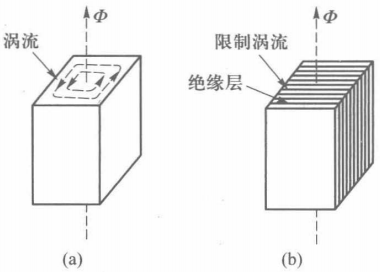
\includegraphics[width = .3\textwidth]{graphics/Screenshot 2025-09-11 at 21.07.39.png}
\caption{涡流损耗}
\label{涡流损耗}
\end{figure}

由上可知,铁心线圈交流电路的有功功率为

\begin{equation}
P = UI \cos \varphi = RI^2 + \Delta P_{\text{Fe}}
\end{equation}

\section{变压器}

\subsection{变压器的工作原理}

\subsubsection{电压变换}

电阻压降和漏磁电动势较小,与主磁电动势比较起来,可以忽略不计。于是

\begin{equation}
    u_1 \approx - e_1 \quad \dot{U_1} \approx - \dot{E_1}
\end{equation}

根据式\ref{16},\(e_1\)的有效值为

\begin{equation}
    E_1 = 4.44 f N_1 \Phi_m \approx U_1
\end{equation}

同理,对二次绕组电路

\begin{equation}
    e_2 = R_2 i_2 + (-e_{\sigma 2}) + u_2
\end{equation}

感应电动势\(e_2\)的有效值为

\begin{equation}
    E_2 = 4.44 f N_2 \Phi_m
\end{equation}

变压器空载时

\begin{equation}
    I_2=0, E_2 = U_{20}
\end{equation}

式中\(U_{20}\)式空载时二次绕组的端电压。

\begin{figure}[!h]
    \centering
    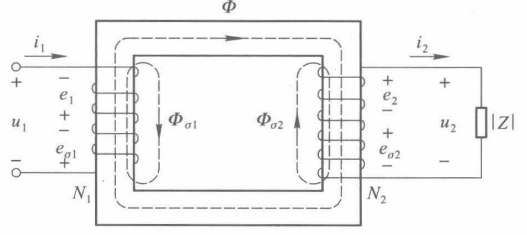
\includegraphics[width = .4\textwidth]{graphics/Screenshot 2025-09-13 at 00.57.19.png}
    \caption{变压器的原理图}
    \label{变压器的原理图}
\end{figure}

一次、二次绕组的电压之比为

\begin{equation}
    \frac{U_1}{U_2} \approx \frac{E_1}{E_2} = \frac{N_1}{N_2} = K
    \label{25}
\end{equation}

式中\(K\)称为变压器的\textbf{变比},亦即一次、二次绕组的匝数比。

\subsubsection{电流变换}

由\(U_1 \approx E_1 = 4.44 f N_1 \Phi_m\)可知,电源电压\(U_1\)和电源频率\(f\)不变时,\(\Phi_m\)近于不变。
这就是说,变压器铁心中主磁通最大值在变压器空载或有载时,基本上是恒定的。那么,这两种状态时的磁通势也应当是近于相等的,即

\begin{equation}
    N_1 \dot{I_1} + N_2 \dot{I_2} \approx N_1 \dot{I_0}
\end{equation}

上式中\(\dot{I_0}\)很小,于是

\begin{equation}
    N_1 \dot{I_1} \approx - N_2 \dot{I_2}
\end{equation}

可以得出

\begin{equation}
    \frac{I_1}{I_2} \approx \frac{N_2}{N_1} = \frac{1}{K}
    \label{28}
\end{equation}

这就是变压器的电流变换作用,即一次、二次绕组电流之比等于它们匝数比的倒数。

\subsubsection{阻抗变换}

根据\ref{25}和\ref{28}可得出

\begin{equation}
    \frac{U_1}{I_1} = \frac{\dfrac{N_1}{N_2}U_2}{\dfrac{N_2}{N_1}I_2} = \left(\frac{N_1}{N_2}\right)^2 \frac{U_2}{I_2}
\end{equation}

于是

\begin{equation}
    \begin{aligned}
        \left|Z^{\prime}\right| & =\left(\frac{N_1}{N_2}\right)^2|Z| \\
        & =K^2|Z|
    \end{aligned}
\end{equation}

\subsection{变压器的外特性}

变压器的外特性如图\ref{变压器的外特性曲线}所示。由特性曲线\(U_2=f(I_2)\)可见,随着二次绕组电流\(I_2\)的增大,输出电压\(U_2\)的下降逐渐明显。
电压变化率

\begin{equation}
\Delta U \%=\frac{U_{20}-U_2}{U_{20}} \times 100 \%
\end{equation}

额定容量

\begin{equation}
    S_N = U_{28} I_{28}
\end{equation}

输出有功功率

\begin{equation}
    P_2 = U_{28} I_{28} \cos \varphi_2
\end{equation}

\begin{figure}[!h]
    \centering
    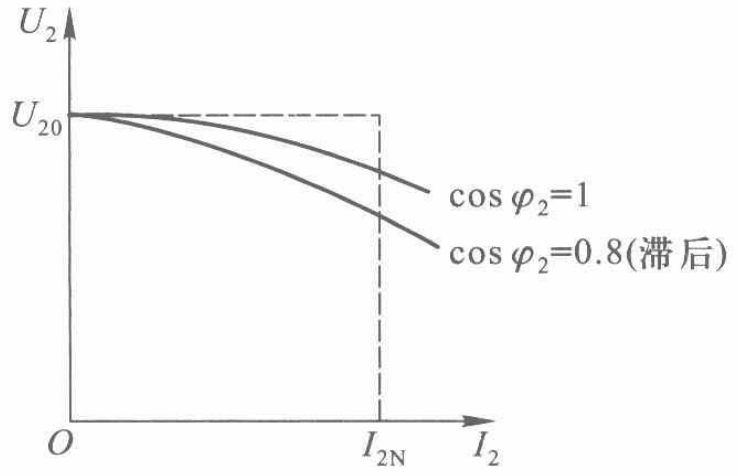
\includegraphics[width = .4\textwidth]{graphics/Screenshot 2025-09-13 at 01.26.07.png}
    \caption{变压器的外特性曲线}
    \label{变压器的外特性曲线}
\end{figure}

\subsection{变压器的损耗与功率}

变压器的效率

\begin{equation}
\eta=\frac{P_2}{P_1}=\frac{P_2}{P_2+\Delta P_{\mathrm{Fe}}+\Delta P_{\mathrm{Cu}}}
\end{equation}

\subsection{特殊变压器}

\subsubsection{自藕变压器}

二次绕组是一次绕组的一部分,则
\begin{equation}
    \frac{U_1}{U_2} = \frac{N_1}{N_2} = K \quad
    \frac{I_1}{I_2} = \frac{N_2}{N_1} = \frac{1}{K}
\end{equation}

\begin{figure}[!h]
    \centering
    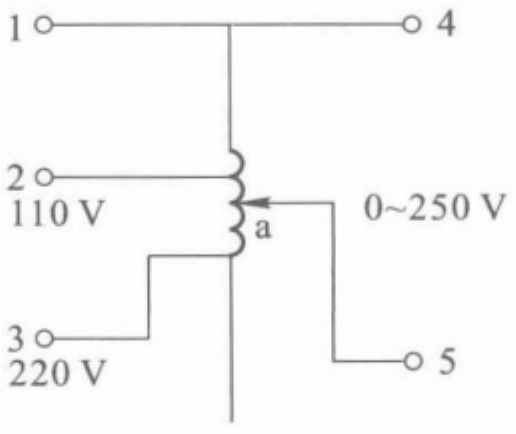
\includegraphics[width = .25\textwidth]{graphics/Screenshot 2025-09-15 at 18.10.20.png}
    \caption{自藕变压器的电路}
    \label{自藕变压器的电路}
\end{figure}

\section{电磁铁}

电磁铁的吸力是它的主要参数之一。直流电磁铁的吸力的大小与气隙的截面积\(S_0\)及气隙中的磁感应强度\(B_0\)的平方成正比。计算吸力的基本公式为
\begin{equation}
    F = \frac{10^7}{8 \uppi} B_0^2 S_0
\end{equation}

交流电磁铁中磁场是交变的,吸力的最大值为
\begin{equation}
    F_m = \frac{10^7}{8 \uppi} B_m^2 S_0
\end{equation}
计算时只考虑吸力的平均值
\begin{equation}
    F = \frac{10^7}{16 \uppi} B_m^2 S_0
\end{equation}

\end{document}
